\begin{figure}
\centering
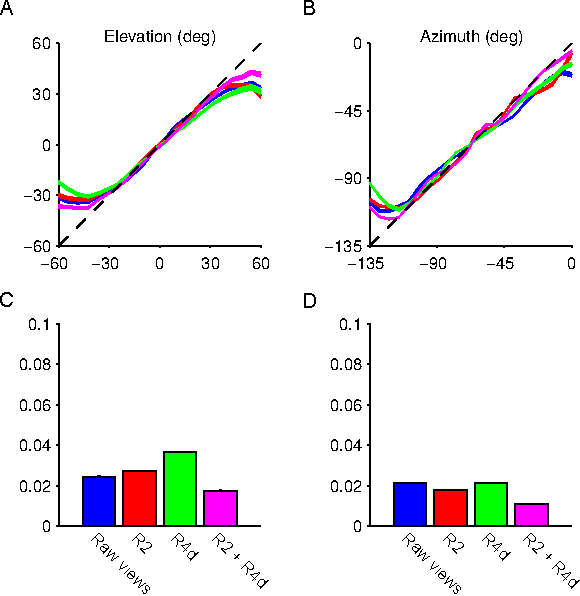
\includegraphics{figures/elaz}
\caption{[PRG 13/8/15] How much positional information is preserved in the R2 population code.
Neural networks were trained to estimate the elevation and azimuth of randomly generated 'blob' stimuli ($N=$~10,000)  from raw views ($N=36$~pixels; blue), R2 neurons ($N=28$; red), R4d neurons ($N=14$; green) or R2 and R4 neurons ($N=42$; magenta). For each visual input a network was trained 100 times and average performance with blobs that were not part of the training set was taken.
A and B: Plots of elevation and azimuth of the test visual stimuli \emph{vs} the mean network output (n=100). The dashed line indicates ideal performance (i.e. $y=x$) and the thickness of the lines at each point shows standard error.
The possible values of elevation and azimuth were constrained by the size of the fruitfly visual field (approx. $120\degree \times 270\degree$). Within this range there were 22 possible values.
C and D: Average network performance (Mean square error) for networks trained to recover elevation (C) or azimuth (D) and for each type of visual input (colour code as above). Standard error is shown, but is very small.
}
\label{fig:elaz}
\end{figure}
